\documentclass[11pt, oneside]{article}   	% use "amsart" instead of "article" for AMSLaTeX format
\usepackage{geometry}                		% See geometry.pdf to learn the layout options. There are lots.
\geometry{letterpaper}                   		% ... or a4paper or a5paper or ... 
%\geometry{landscape}                		% Activate for for rotated page geometry
%\usepackage[parfill]{parskip}    		% Activate to begin paragraphs with an empty line rather than an indent
\usepackage{graphicx}				% Use pdf, png, jpg, or eps§ with pdflatex; use eps in DVI mode
								% TeX will automatically convert eps --> pdf in pdflatex		
\usepackage{amssymb}

\title{Heuristic Analysis: Online Shopping}
\author{Edward Bramanti}

\begin{document}
\maketitle
\section{Amazon}
\subsection{Test 1}
As can be seen from the usability metrics, Amazon scored well in efficiency and satisfaction, while matching both in learnability. I believe that Amazon has experienced these results for a few reasons, which are listed below.
\subsubsection{User Memory Load too High}
Nielsen's Usability Heuristics discuss that minimizing the user's memory load is highly important to a usable system. Nevertheless, Amazon would consistently make it difficult to get from one point to the other. Searching for a flash drive is an explosion of information and ratings, while eBay and Shopzilla take a simpler approach of focusing on purchase. In addition, pop-ups some users experienced about Amazon Prime would further increase the amount of things a user would have to think about before reaching checkout.
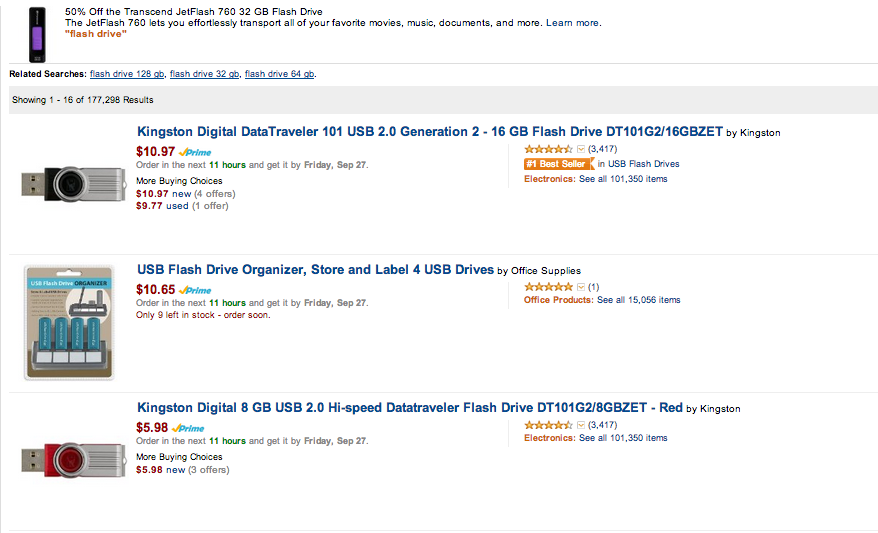
\includegraphics[width=6in, height=2.96in]{Amazon1}
\subsection{Test 2}
Amazon outscored eBay and found great success in learnability and satisfaction. Nevertheless, efficiency suffered, even compared to eBay's clunky credit card system (more on that later.) Listed is an important reason why efficiency took a big hit on Amazon's credit card section.
\subsubsection{A disconnect between the developer/user mental model}
Amazon website designers understood that approaching account options in a way that encompasses everything that the user needs is important so that the user can succinctly perceive the task they want to accomplish. The problem is that the user's view of the system image(in this case, the My Account Page) can become convoluted by the sheer number of options (pictured below.)

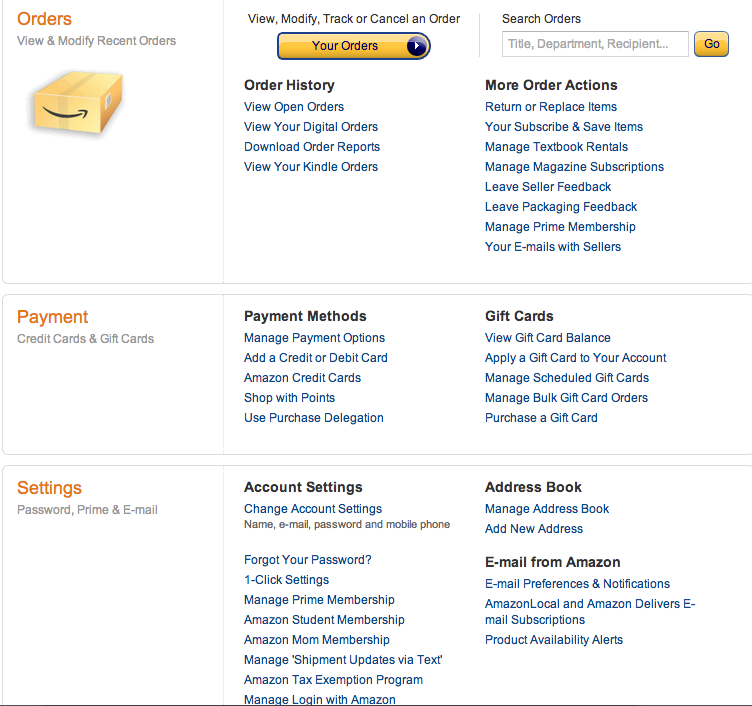
\includegraphics[width=6in, height=4.5in]{Amazon2}

Users would gravitate towards the payment section (highlighted in orange in the above graphic), but a disconnect between designer and user begins. The user would see the add credit card, and be able to successfully add. But, when they needed to delete a credit card, users would go to the "Add Credit Card" section and attempt to remove from there. Since credit card is what most users were looking for to complete the task, they would make an error and look in the entirely wrong section. Even though the "Add Credit Card" section clearly does not say delete, users would view the word "Credit Card" and instantly be drawn to the option. Amazon's web developers thought that the logical thing to do if you wanted to modify payment options would be "Manage Payment Options," but they also include a credit card adding option outside of that context. This is one of the biggest reasons why efficiency will suffer if someone desires to delete their credit card: instead of clicking "Manage Payment Options," they will be drawn to the word they have formulated in their mind (in this case, "credit card").

\subsection{Test 3}
Referencing the metrics taken, Amazon suffered in learnability as well as efficiency when it came to using the sidebar to find the Nokia Lumia 920.
\subsubsection{Lack of efficient information to be assimilated by the user}
One of the organizational guidelines for data display, published by Smith and Mosier in 1986, is that data must be efficiently assimilated by the user. In the study done when users were asked to find the Lumia 920 using only department selection, and narrowing results with the sidebar, this is what would occur after their first click.

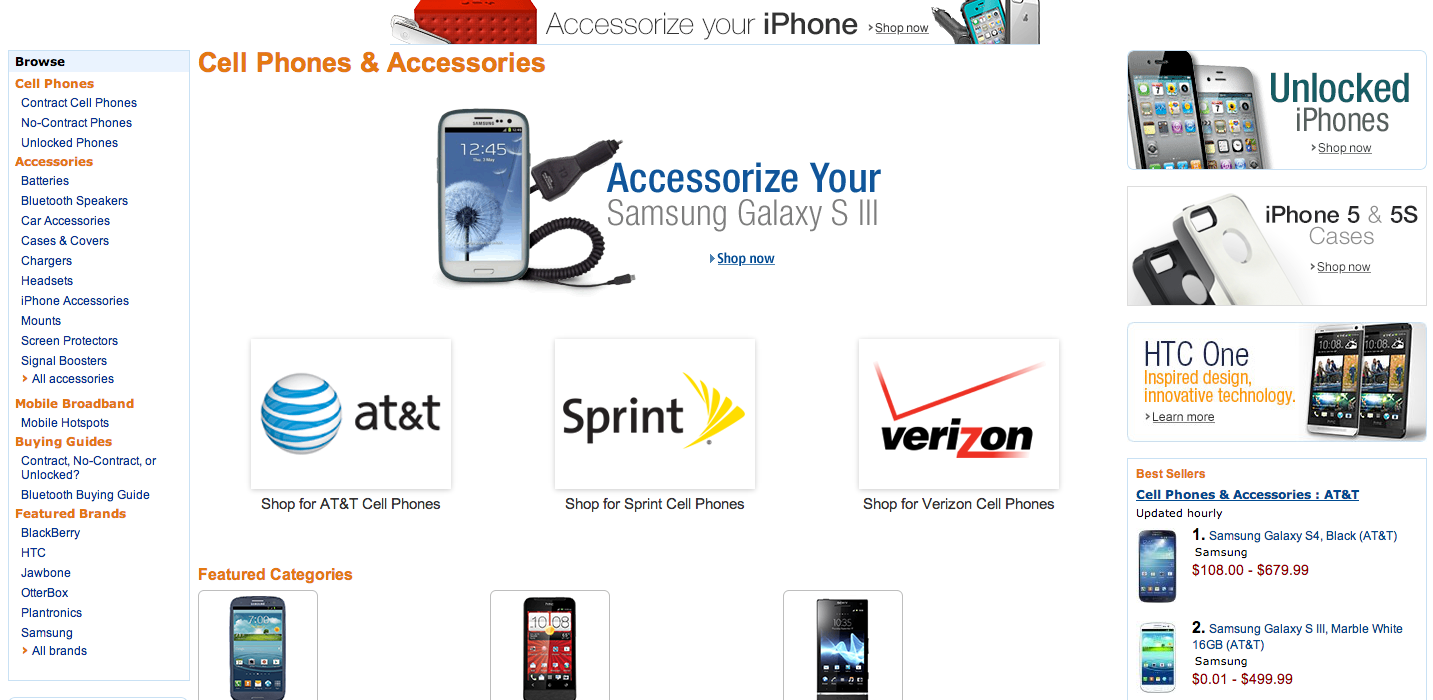
\includegraphics[width=6in, height=3.4in]{Amazon3}

After looking at just the cell phones and accessories page, it becomes clear how inefficient Amazon's department search is. There are so many ways to narrow down the options that the user does not know where to begin. For example, the Nokia Lumia 920 is an AT\&T phone. It is sold with a contract, and it also can be sold unlocked as well. That presents two options to the users, but neither of those are part of the title. While there is plenty of information displayed, featured brands does not even list a "Nokia" option unless you scroll further down the page, which forces the user deeper into convolution. I conclude this point by saying that there is a lack of presentable data that assists the user with finding what they want from shopping online over looking through a store.
\section{eBay}
\subsection{Test 1}
Looking at this test, eBay surprisingly returned a high level of satisfaction, efficiency and learnability while searching for a USB flash drive. Below, I explain the reason why these results are a product of eBay's simplicity.
\subsubsection{Simplifies interface knowledge to empower the user}

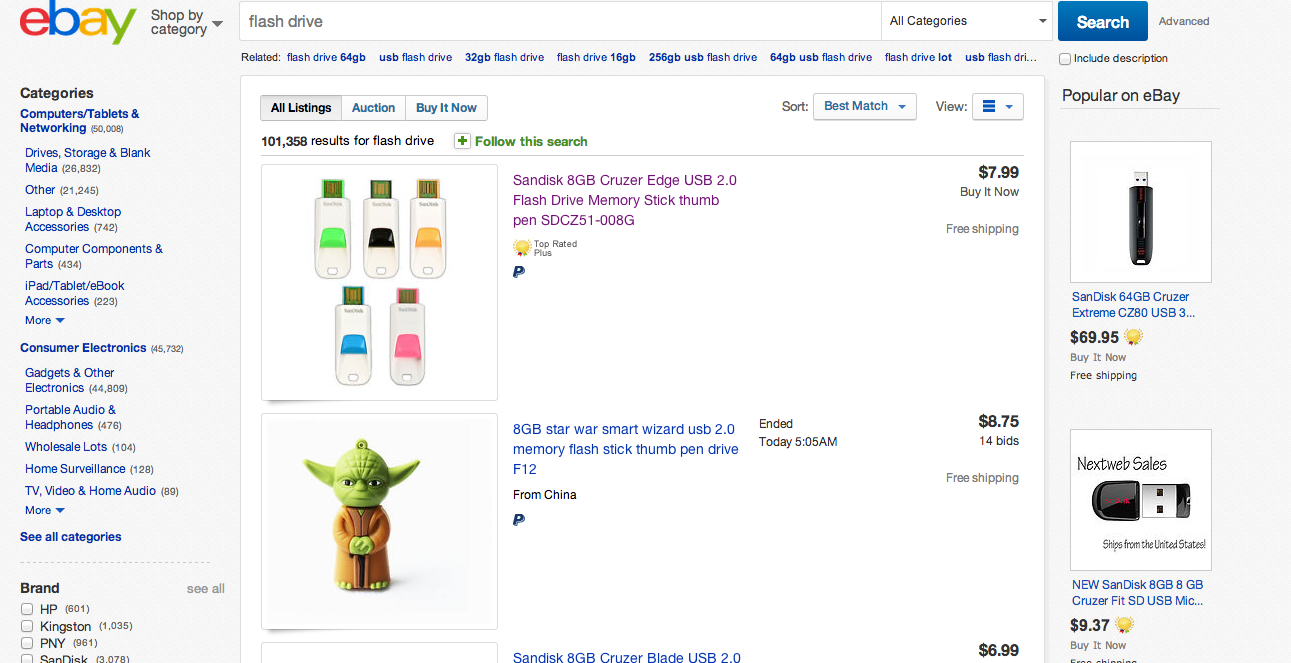
\includegraphics[width=6in, height=3.4in]{eBay1}
eBay has designed their user interface to be incredibly easy to understand. It puts the focus on what you actually want: the item, and the item's options, as quickly and simplistically as possible. eBay's system image is one that has grabbed the satisfaction of users because it provides powerful tools which do not clutter the beautifully designed interface. In addition to this, eBay has taken a page from Amazon by adding a cart option, which allows users to queue up multiple items. And while this interface caters to novices just looking to buy something quickly, eBay's power in its interface quickly becomes clear when simple sort functions appear on the top, and more advanced ones appear as you scroll (as most users will when looking for a good price or niche product).

\subsection{Test 2}
eBay struggles when it comes to credit cards. Since PayPal is designed to be like a bank account, but requires a credit card to set up, it makes it difficult to manually add a credit card. I will detail the interface problems below.
\subsubsection{eBay's payment methods do not cater to universal usability}
In almost every case of the tests we ran to determine how usable a credit card is on eBay, the user would have difficulty interpreting the system image and how to reach a point where they could select a credit card instead of a PayPal account. Why? Because they would FIRST have to select PayPal as a payment method in order to use PayPal as a guest!
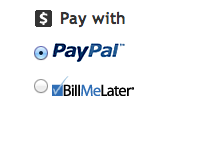
\includegraphics[width=2in, height=1.5in]{eBay2}
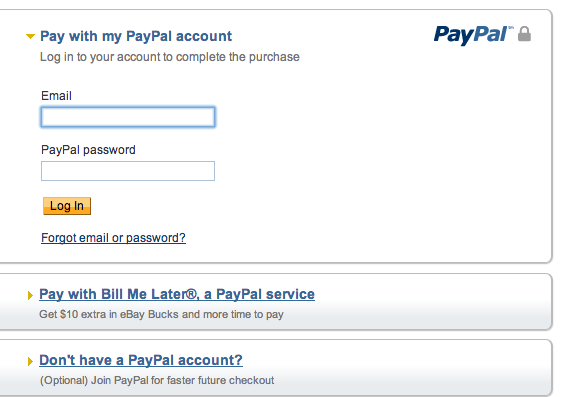
\includegraphics[width=4in, height=3in]{eBay3}
As you can see in the image on the right, "Don't have a PayPal account?" only shows up after the user has selected Pay with PayPal. This led to a lack of user control as they became frustrated trying to find a method to continue forward. While I believed at first that this was a disconnect between the system the developer is creating and the system image the user is perceiving, in my later part of the study I found that certain eBay users have an actual credit card selector available to them!

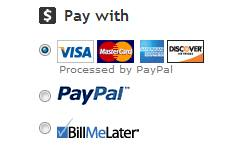
\includegraphics[width=2in, height=1.5in]{eBay4} 

It was incredible to find out that there was an actual method to attain this. But, it was only available to one out of the five users tested. This is clearly a lack of universal usability; eBay expects their users to guess their way to a process while some users get the ease of access that would make sense to their perception of the system image.
\subsection{Test 3}
While eBay provided an ease of learnability, it lacked efficiency and satisfaction. Below I will outline the reasons why finding a Lumia 920 on eBay can be a cumbersome process.
\subsubsection{A need for universal usability mixed with Fitt's Law}
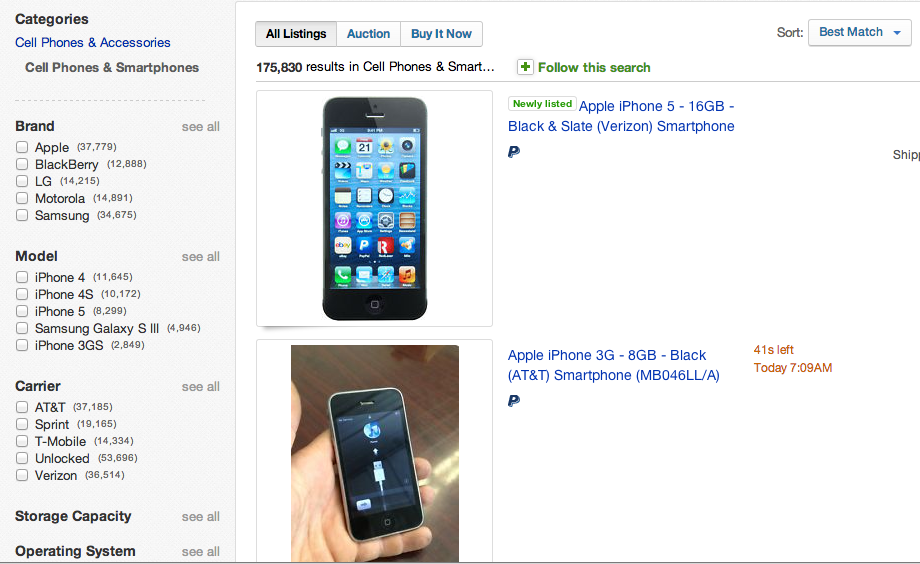
\includegraphics[width=6in, height=3.5in]{eBay5}
Seen above is an example of a cell phone search by department. Clearly, a few of the top brands can be seen. This definitely caters to novices, while also providing a "see all" option for users with more experience. The problem is if a novice user is looking for a phone that is not listed in those options, the size of "see all" when considered with Fitt's Law demonstrates the lack of efficiency for users searching for the Nokia Lumia 920. Some did not even see the option at all in our Usability Testing, which leads me to believe that both universal usability and Fitt's Law are the solution to the problem. The power of the sidebar is there, and the web developers at eBay have built a powerful system; now, it is their job to improve the system image for their users.
\section{Shopzilla}
\subsection{Test 1}
Shopzilla's interface to comply with Test 1's search for a flash drive was easy to learn, but suffers from a lack of efficiency and satisfaction. Below, I detail why the interaction of the user with Shopzilla is at times difficult.
\subsubsection{A lack of organization in Shopzilla's aggregation}
Shopzilla's job is to aggregate results from multiple shopping sites to provide a wealth of information for the consumer, informing them and allowing them to buy the product they want at the best price. Aggregate shopping websites, such as Google Shopping, work well for certain items. Nevertheless, Shopzilla suffer from flaws in their own display of data and their compilation of multiple websites into their search results. Many of the users in testing had trouble finding a flash drive they wanted, as results that returned from their search would lead to website results with non-working links, or provided returned results that did not match the search term. This led to frustration, and caused an extreme decline in user satisfaction. They felt powerless as the automated search returned results that were irrelevant to their goals. It also hindered efficiency, as users spent more time scrolling to find a result that matched what they were looking for (in this case, some form of flash drive).
\subsection{Test 2}
Test 2 on Shopzilla was not performed because this is a point that should strictly be addressed using heuristic analysis. The reason why is due to the fact that Shopzilla does not support any form of payment methods; it links to other stores while compiling a list of all possible items online matching your search result. If one considers the endless amount of shopping websites, it brings into clarity the sheer amount of times you may have to reenter your information while shopping on Shopzilla. I believe that this presents a problem to the user, in the context of the Stages-of-Action Theory. There is a "gulf in execution"; that the user wants to be able to have a way to purchase easily from all of these sites, but they don't understand the possibility that Shopzilla could act as a bridge to pay instead of re-entering your information endlessly. Using these principles, Shopzilla could actually implement a payment method that would make it easier for users to purchase items while still maintaining a philosophy of aggregated shopping results. 
\subsection{Test 3}
In Test 3, Shopzilla had average to poor scores in learnability and satisfaction, but the best score in efficiency. I will explain why I believe the results were this way searching departmentally was more efficient for Shopzilla at the cost of learnability and satisfaction.
\subsubsection{The Kitchen-Sink Approach without the Joy of Use}
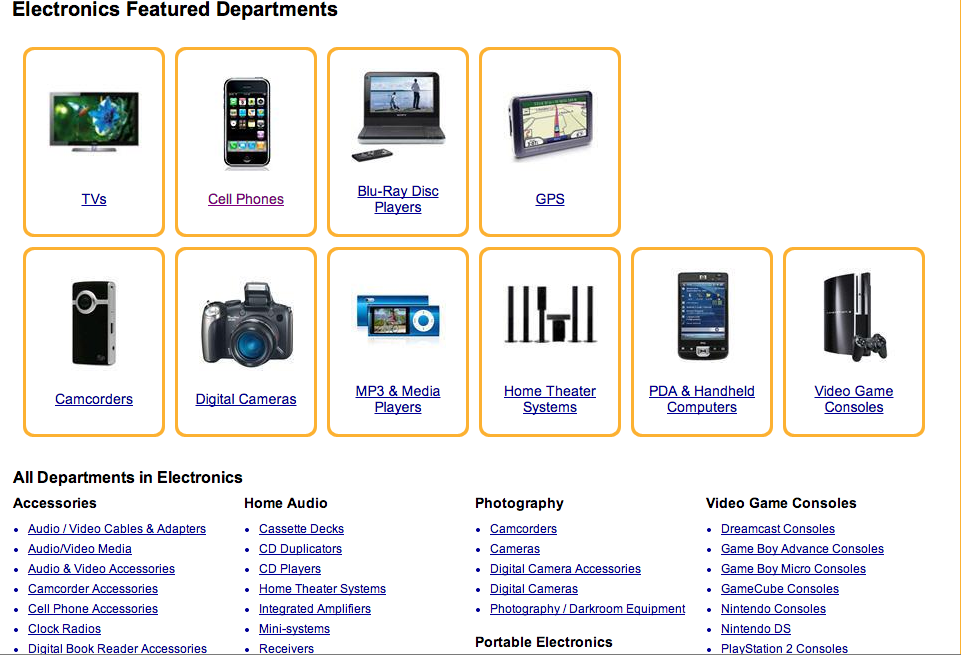
\includegraphics[width=6in, height=3.5in]{Shopzilla1}
Shopzilla has clearly designed a user interface based on endless options and endless parameters at the expense of satisfaction. The user interface is very basic-looking, and is filled with boring text, photos, and colors. Shopzilla's boring design is powerful for the user, if they utilize it correctly. It's just not particularly satisfying, and it makes it difficult for the user to form a good conceptual model of how they want to approach the task. If Shopzilla improves the graphical user interface of their site, it will result in a drastic improvement in learnability and satisfaction, and will continue to improve on the great efficiency already proven and recorded in the Usability Study.
\section{Conclusion}
To conclude, I believe there are ways each online shopping site can improve. With Amazon, I believe adding some kind of virtualized "WindowShop" mode will provide the user with a department search that feels like actually shopping at a brick-and-mortar store, solving the problems of the Lumia 920 test. With eBay, making credit cards through PayPal a more prominent option and providing an interface that utilizes universal usability and Fitt's Law will go a long way to improve the lacking pay experience. And with Shopzilla, a strong GUI redesign for the department section as well as a payment system where Shopzilla handles the transaction would improve the user experience.


\end{document}  